%%%%%%%%%%%%%%%%%%%%%%%%%%%%%%%%%%%%%%%%%%%%%%%%%%%%%%%%%%%%%%%%%
% Beamer Presentation Code - FINAL VERSION 25.0 (Definitive & Corrected)
%
% --- CRITICAL FIX ---
% 1. RESTORED DELETED CONTENT: The four "Regional Layout Analysis" slides
%    were mistakenly deleted in the previous version. They have been fully restored.
% 2. CORRECT INSERTION: The "System GMM" slides have been correctly inserted
%    AFTER the "Mechanism Analysis (Summary)" slide, without altering any
%    other part of the presentation.
%
% I sincerely apologize for the previous error. This version is correct.
%%%%%%%%%%%%%%%%%%%%%%%%%%%%%%%%%%%%%%%%%%%%%%%%%%%%%%%%%%%%%%%%%

\documentclass[aspectratio=169]{beamer}

\usepackage[utf8]{inputenc}
\usepackage{heuristica}
\usepackage[T1]{fontenc}
\usepackage[heuristica,vvarbb,bigdelims]{newtxmath}
\renewcommand*\oldstylenums[1]{\textosf{#1}}
\usepackage[sfdefault,scaled=.85]{FiraSans}
\usepackage{graphicx}
\usepackage[english]{babel}
\usepackage[pages=some]{background}
\usepackage{amsmath}
\usepackage{caption} 
\usepackage{booktabs} 

\pagenumbering{arabic}

\definecolor{mostazaccm}{RGB}{218, 165, 32} 

\newtheorem{hypothesis}{Hypothesis}
\newtheorem{teorema}{Theorem}

% Title adjusted for better display in 16:9
\title{ 
  \huge\textbf{The Cybernetic Teammate} \\ 
  {\color{mostazaccm} \large A Field Experiment on Generative AI and Teamwork}
}
\author{Yingkai Hua, Taoran Li, Lujie Zhang, Yi Sun}
\date{Selected Paper Reading for Basic Theory of Smart Goverance} 
\institute{School of Smart Goverance, Rermin University of China}

\usetheme{ccm4}

% --- GLOBAL FONT & HEADLINE ADJUSTMENTS ---
\setbeamerfont{normal text}{size=\small}
\setbeamerfont{block body}{size=\small}
\setbeamerfont{block title}{size=\normalsize}

% Headline with doubled height
\setbeamercolor{section in head/foot}{fg=white, bg=rojotexto} 
\setbeamertemplate{headline}
{
  \leavevmode%
  \hbox{%
    \begin{beamercolorbox}[wd=\paperwidth,ht=5.0ex,dp=2.2ex,center]{section in head/foot}%
      \usebeamerfont{section in head/foot}
      \insertsectionnavigationhorizontal{\paperwidth}{\hskip0.02\paperwidth}{\hskip0.02\paperwidth}
    \end{beamercolorbox}%
  }%
  \vskip-0.2pt 
}

% Background setup for all slides
\backgroundsetup{contents=
\includegraphics[width=\paperwidth,height=\paperheight]{images/FONDO AL 10.png}}

\begin{document}

% Title Page
{
\setbeamertemplate{background}{
  
\includegraphics[width=\the\paperwidth,height=\the\paperheight]{images/P4.png} 
}
\begin{frame}[plain]
  \titlepage 
\end{frame}
}

% Outline Frame
\begin{frame}
  \frametitle{Outline}
  \tableofcontents
\end{frame}

% --- SECTION 1: INTRODUCTION ---
\section{Introduction}

\begin{frame}
  \frametitle{Motivation: The Rise of the Digital Economy}
  \begin{itemize}
    \item \textbf{Global Context:} A global consensus is forming on the new digital revolution, pushed by factors like globalization and the pandemic.
    \item \textbf{China's Strategy:} Actively promoting digital industrialization and the digital transformation of traditional industries.
    \item \textbf{The Productivity Puzzle:} While China's Total Factor Productivity (TFP) is growing, it still lags behind developed nations.
    \vspace{1em}
    \item<2-> \textbf{Core Question:} How does Digital-Intelligent Transformation (DIT) enhance enterprise TFP? The answer may lie within the firm's governance.
  \end{itemize}
\end{frame}

\begin{frame}
  \frametitle{Literature and Research Gaps}
  \begin{block}{What We Know}
    \begin{itemize}
        \item DIT can modernize processes and improve decision-making.
        \item Technologies like AI, Blockchain, and Big Data can reduce costs and optimize resources.
        \item The impact of DIT is not uniform across all firms (depends on life cycle, region, etc.).
    \end{itemize}
  \end{block}
  \begin{alertblock}{What We Don't Know (Research Gaps)}
    \begin{enumerate}
        \item \textbf{The "Black Box":} How do internal governance structures (board, pay, ownership) \textit{mediate} the DIT-TFP link?
        \item \textbf{Firm Heterogeneity:} How do these effects differ by region, ownership, and factor intensity?
    \end{enumerate}
  \end{alertblock}
\end{frame}

\begin{frame}
  \frametitle{Hypotheses Development}
  \begin{hypothesis}[H1]
    DIT has a positive impact on enterprise TFP.
  \end{hypothesis}
  \vfill
  \begin{hypothesis}[H2]
    DIT improves TFP by increasing the proportion of female executives.
  \end{hypothesis}
  \vfill
  \begin{hypothesis}[H3]
    DIT improves TFP by reducing the average age of management.
  \end{hypothesis}
  \vfill
  \pause
  \begin{block}{Other Hypotheses}
  DIT also boosts TFP through higher DSE compensation, reduced ownership-control separation, and increased board network centrality.
  \end{block}
\end{frame}

% --- SECTION 2: THEORETICAL MODEL ---
\section{Theoretical Model}

\begin{frame}
  \frametitle{Theoretical Model: Basic Assumptions}
    \begin{block}{Economy Structure}
        A three-sector economy is assumed:
        \begin{itemize}
            \item \textbf{Government:} Collects taxes, invests in digital-intelligent capital ($M_t$).
            \item \textbf{Enterprises:} Produce final goods using a mix of inputs.
            \item \textbf{Households:} Supply labor and consume.
        \end{itemize}
    \end{block}
    \begin{block}{Labor and Capital Types}
        To capture the effects of DIT, we distinguish between:
        \begin{itemize}
            \item \textbf{Labor:} High-skilled ($L_H$) and Low-skilled ($L_L$).
            \item \textbf{Capital:} Digital-Intelligent ($M_t$) and Productive Physical ($K_P$).
        \end{itemize}
    \end{block}
\end{frame}

\begin{frame}
  \frametitle{Theoretical Model: Production Function}
  \begin{block}{Multi-Nested CES Production Function}
  The final product $Y_t$ is a combination of two intermediate inputs:
  \end{block}
  \begin{equation}
    Y_{t} = \left[ \theta_{t} (A_{t} Y_{K,H,M,t})^{\frac{\sigma-1}{\sigma}} + (1-\theta_{t}) (B_{t} L_{L,t})^{\frac{\sigma-1}{\sigma}} \right]^{\frac{\sigma}{\sigma-1}} \label{eq:main_prod_full}
  \end{equation}
  where the first input, $Y_{K,H,M,t}$, is itself a CES aggregate of high-skilled labor and two types of capital:
  \begin{equation}
    Y_{K,H,M,t} = \left[ \phi_t (C_t K_{P,t})^{\frac{\rho-1}{\rho}} + \psi_t (D_t M_t)^{\frac{\rho-1}{\rho}} + (1-\phi_t-\psi_t)(E_t L_{H,t})^{\frac{\rho-1}{\rho}} \right]^{\frac{\rho}{\rho-1}}
  \end{equation}
  \begin{itemize}
    \item $\sigma$: elasticity of substitution between high-skilled and low-skilled bundles.
    \item $\rho$: elasticity of substitution among capital and high-skilled labor.
  \end{itemize}
\end{frame}

\begin{frame}
  \frametitle{Theoretical Model: TFP Growth Derivation}
  \begin{block}{Profit Maximization and First-Order Conditions (F.O.C.s)}
    Firms maximize profit, leading to F.O.C.s where factor prices equal their marginal products. For example, for high-skilled labor ($L_H$):
    \begin{equation*}
       w_{H,t} = \frac{\partial Y_t}{\partial L_{H,t}}
    \end{equation*}
  \end{block}
  
  \begin{alertblock}{Key Result: TFP Growth Rate}
  After decomposing economic growth, the TFP growth rate ($\widehat{TFP}_t$) is derived as:
    \begin{equation}
        \widehat{TFP}_{t} = \sum_{j \in \{K,H,M,L\}} s_{j,t} \widehat{A}_{j,t} + \text{Bias Terms}
    \end{equation}
  \end{alertblock}
  This shows TFP growth depends on factor-augmenting technological progress ($\widehat{A}_{j,t}$), factor shares ($s_{j,t}$), and biases from technology and factor allocation.
\end{frame}

% --- SECTION 3: METHODOLOGY ---
\section{Methodology}

\begin{frame}
  \frametitle{Conceptual Framework: The Transmission Mechanism}
  \begin{columns}[T]
    \begin{column}{0.55\textwidth}
      \centering
      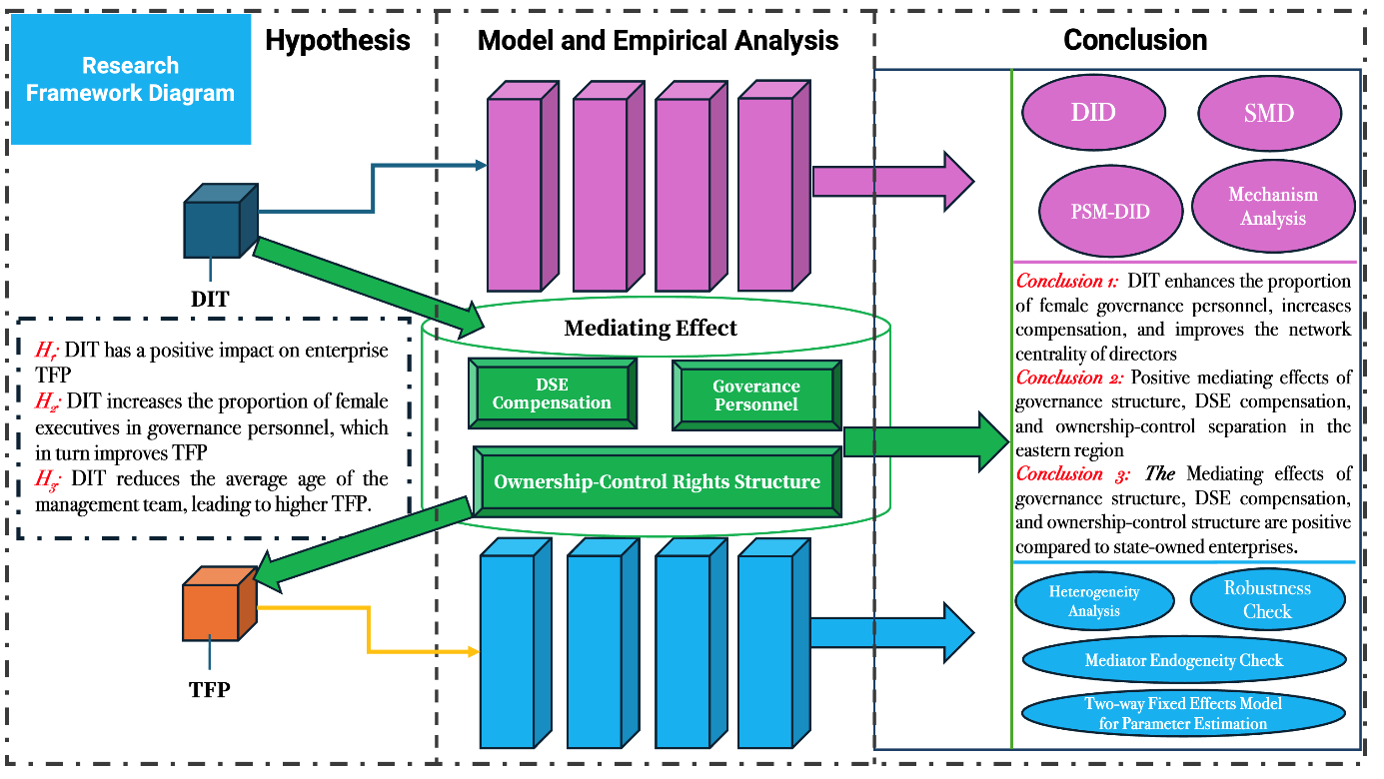
\includegraphics[width=0.95\textwidth]{images/conceptual_framework.png}
      \captionof{figure}{\tiny The DIT \(\rightarrow\) Governance \(\rightarrow\) TFP Pathway}
    \end{column}
    \begin{column}{0.45\textwidth}
      \begin{alertblock}{Transmission Mechanism}
        Our framework models how DIT impacts TFP via two pathways:
        \begin{itemize}
            \item<2-> \textbf{Direct Effect:} DIT directly improves operational efficiency.
            \item<3-> \textbf{Indirect (Mediating) Effect:} DIT drives TFP gains by reshaping governance, through channels like:
                \begin{itemize}
                  \item<4-> \textbf{Personnel Structure:} Optimizing team (age, gender).
                  \item<5-> \textbf{DSE Compensation:} Aligning incentives.
                  \item<6-> \textbf{Ownership Structure:} Enhancing oversight.
                \end{itemize}
        \end{itemize}
      \end{alertblock}
    \end{column}
  \end{columns}
\end{frame}

\begin{frame}
  \frametitle{Methodology: Variables}
    \begin{columns}[T]
        \begin{column}{0.5\textwidth}
            \begin{block}{Dependent Variable}
                \begin{itemize}
                    \item \textbf{TFP:} Total Factor Productivity, measured via the Ackerberg, Caves, Frazer (ACF) method.
                \end{itemize}
            \end{block}
            \begin{alertblock}{Mediating Variables}
                \begin{itemize}
                    \item \textbf{Personnel:} Female exec ratio (\textit{fman}), Mgmt age (\textit{mage}).
                    \item \textbf{Compensation:} DSE pay (\textit{mwage1-3}).
                    \item \textbf{Ownership:} Separation rate (\textit{devia}), Network centrality (\textit{netm}).
                \end{itemize}
            \end{alertblock}
        \end{column}
        \begin{column}{0.5\textwidth}
            \begin{block}{Core Explanatory Variable}
                \begin{itemize}
                    \item \textbf{DIT:} A dummy variable based on text analysis of annual reports, patents, and government procurement for keywords like "AI", "Big Data", "Blockchain".
                \end{itemize}
            \end{block}
            \begin{block}{Control Variables}
                \begin{itemize}
                    \item \textbf{Firm-level:} Age, R\&D, Lerner Index, Financial Constraints, Debt Ratio.
                    \item \textbf{Industry & Region:} Relevant controls.
                \end{itemize}
            \end{block}
        \end{column}
    \end{columns}
\end{frame}

\begin{frame}
  \frametitle{Methodology: Empirical Model}
  \begin{block}{Strategy: Propensity Score Matching + DID}
  We first use PSM to construct a valid control group, then apply a Difference-in-Differences model to estimate the causal effect.
  \end{block}
  
  \textbf{Main Effect Model:}
  \begin{equation}
     TFP_{it} = \alpha_0 + \alpha_1 \textbf{Dit}_{it} + \mathbf{X'_{it}}\mathbf{\Gamma} + \mu_i + \lambda_t + \epsilon_{it}
  \end{equation}
  \begin{itemize}
    \item $Dit_{it}$ is the core interaction term ($treat_i \times post_t$).
    \item $\mu_i$ & $\lambda_t$ are individual and time fixed effects.
  \end{itemize}
  \vfill
  \textbf{Mediation Effect Models (3-step approach):}
  \begin{align}
    TFP_{it} &= \gamma_1 Dit_{it} + ... + \epsilon_{1it} \quad (\text{Total Effect}) \\
    Mediator_{it} &= \beta_1 Dit_{it} + ... + \epsilon_{2it} \quad (\text{Path A}) \\
    TFP_{it} &= \gamma'_1 Dit_{it} + \gamma_2 Mediator_{it} + ... + \epsilon_{3it} \quad (\text{Path B + Direct Effect})
  \end{align}
\end{frame}

% --- SECTION 4: EMPIRICAL RESULTS ---
\section{Empirical Results}

\begin{frame}
  \frametitle{Results: Pre-Analysis Checks}
    \begin{block}{Parallel Trend Test}
        The crucial parallel trend assumption holds. TFP trends for treatment and control groups were statistically indistinguishable before DIT implementation.
    \end{block}
    \begin{block}{PSM Covariate Balance}
        After 1:2 nearest-neighbor matching, standardized mean differences for all matching variables are well within the acceptable range, ensuring group comparability.
    \end{block}
\end{frame}

\begin{frame}[fragile]
  \frametitle{Results: Pre-Analysis Checks (Visual Evidence)}
  \begin{columns}[T]
    \begin{column}{0.5\textwidth}
      \begin{block}{Parallel Trend Test Results}
        \centering
        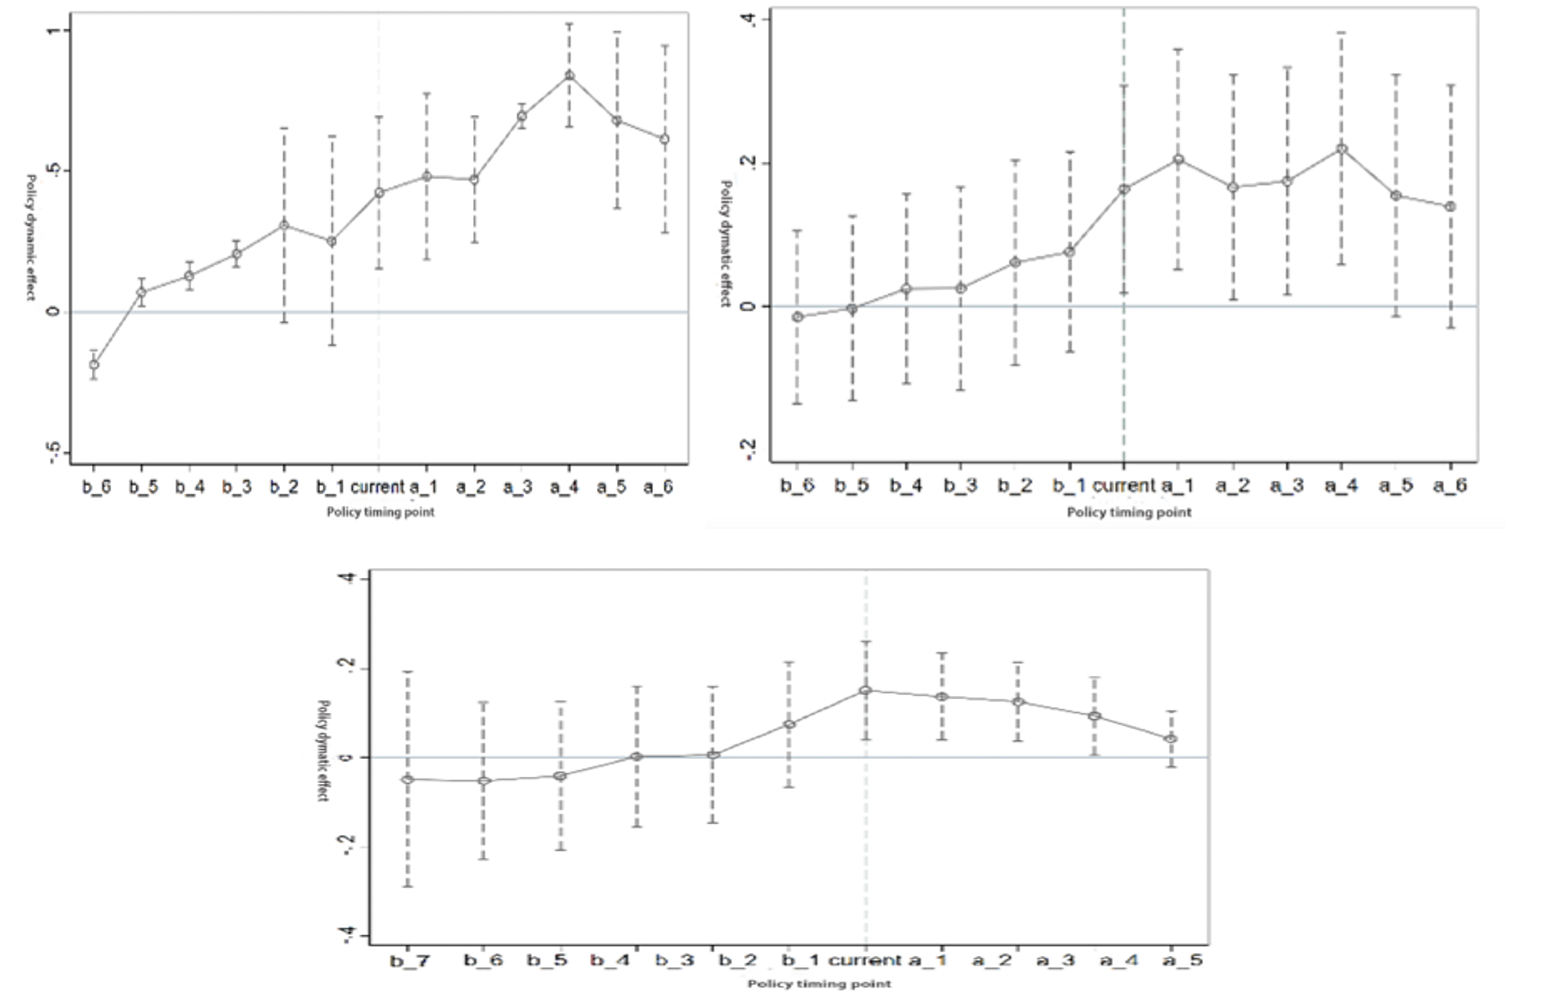
\includegraphics[width=0.9\linewidth]{images/parallel_trend_plot.png}
        \par\medskip
        \tiny
        There is no significant difference in pre-treatment trends. Post-treatment, the treatment group shows a \textcolor{red}{significant and sustained increase in TFP}. This confirms the validity of the DID framework.
      \end{block}
    \end{column}
    \begin{column}{0.5\textwidth}
      \begin{block}{Covariate Balance Test Results}
        \centering
        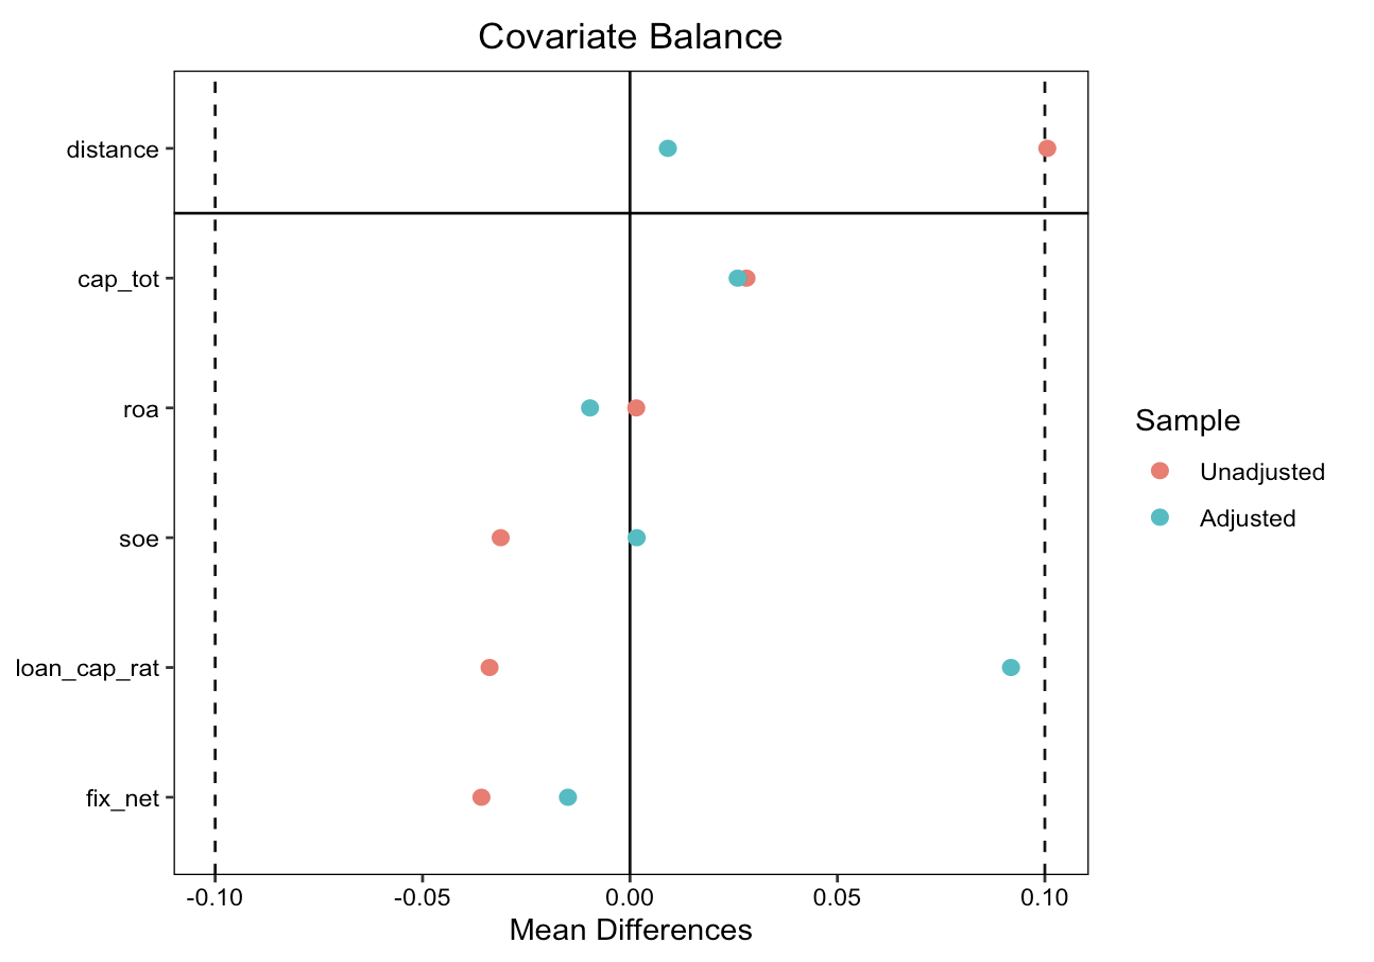
\includegraphics[width=0.9\linewidth]{images/covariate_balance_plot.png}
        \par\medskip
        \tiny
        Before matching, significant imbalances existed. After matching, mean differences for most covariates fall within the acceptable range. \textcolor{red}{This demonstrates that PSM successfully balanced the covariates}, providing a solid foundation for DID estimation.
      \end{block}
    \end{column}
  \end{columns}
\end{frame}

% --- REGIONAL ANALYSIS SLIDES (RESTORED) ---
\begin{frame}
    \frametitle{Regional Layout Analysis: TFP Differences}
    \begin{columns}[T]
        \begin{column}{0.6\textwidth}
            \centering
            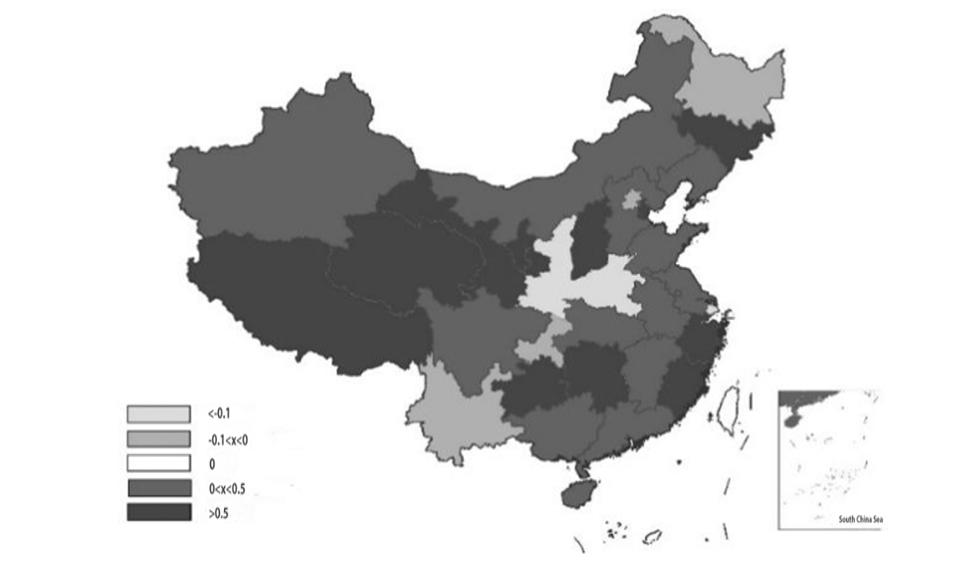
\includegraphics[width=0.9\linewidth]{images/map_tfp.png}
            \captionof{figure}{\tiny Fig 6: TFP Difference (DIT vs. Non-DIT)}
        \end{column}
        \begin{column}{0.4\textwidth}
            \begin{alertblock}{Main Finding}
                The map shows the TFP premium for firms that underwent DIT.
                \begin{itemize}
                    \item Darker shades indicate a larger positive TFP premium.
                    \item \textcolor{red}{In most regions, especially the eastern coastal areas, DIT firms exhibit significantly higher TFP} than their non-DIT counterparts.
                \end{itemize}
            \end{alertblock}
        \end{column}
    \end{columns}
\end{frame}

\begin{frame}
    \frametitle{Regional Layout Analysis: Governance Personnel}
    \begin{columns}[T]
        \begin{column}{0.6\textwidth}
            \centering
            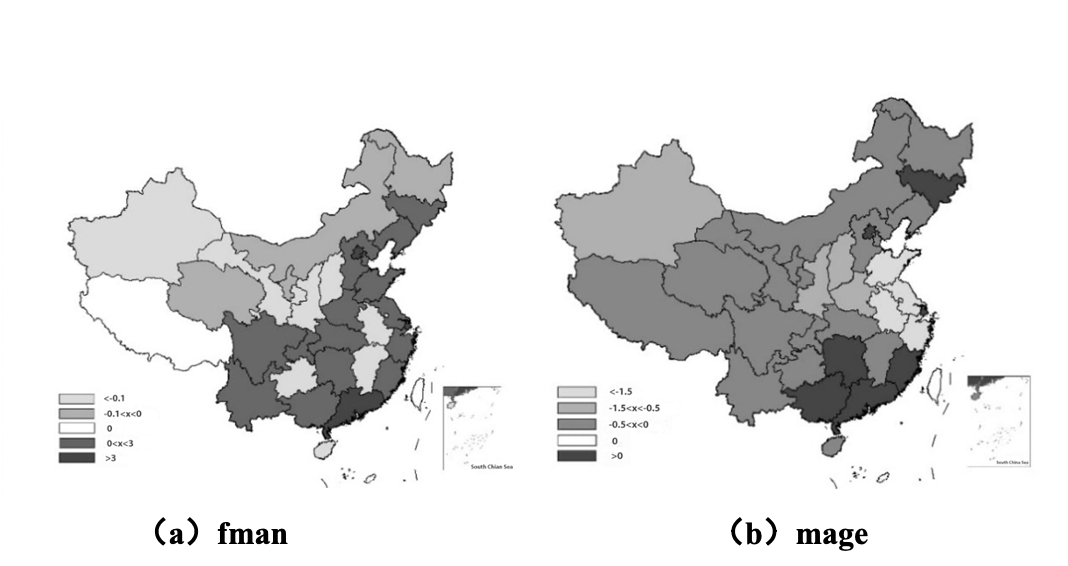
\includegraphics[width=\linewidth]{images/map_personnel.png}
            \captionof{figure}{\tiny Fig 7: Differences in (a) Female Execs \& (b) Mgmt Age}
        \end{column}
        \begin{column}{0.4\textwidth}
            \begin{alertblock}{Main Finding}
                These maps show where DIT firms are more likely to have a higher proportion of female executives (\textit{fman}) and a younger management team (\textit{mage}).
                \begin{itemize}
                    \item The trend is most pronounced in the \textcolor{red}{eastern and central regions}.
                    \item This suggests DIT's impact on personnel structure is geographically concentrated.
                \end{itemize}
            \end{alertblock}
        \end{column}
    \end{columns}
\end{frame}

\begin{frame}
    \frametitle{Regional Layout Analysis: DSE Compensation}
    \begin{columns}[T]
        \begin{column}{0.6\textwidth}
            \centering
            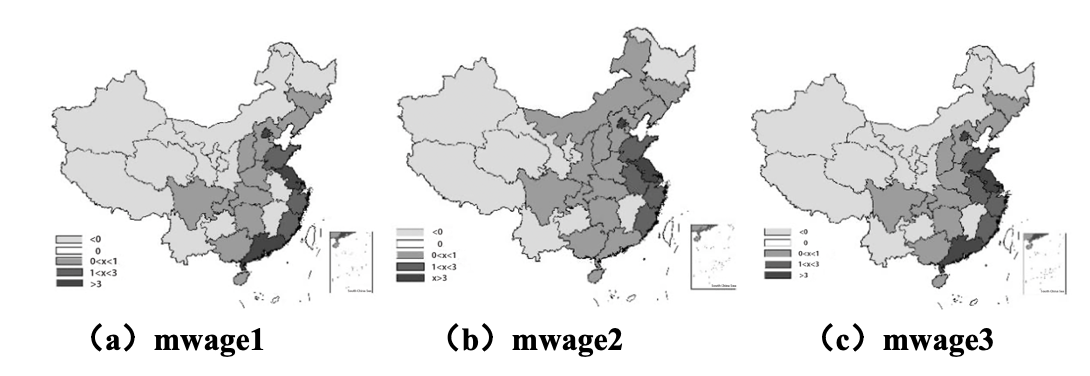
\includegraphics[width=\linewidth]{images/map_compensation.png}
            \captionof{figure}{\tiny Fig 8: Differences in DSE Compensation}
        \end{column}
        \begin{column}{0.4\textwidth}
            \begin{alertblock}{Main Finding}
                These maps illustrate the difference in executive compensation levels between DIT and non-DIT firms.
                \begin{itemize}
                    \item DIT firms in the \textcolor{red}{eastern and most central regions} are significantly more likely to offer higher compensation to their Directors, Supervisors, and Executives.
                \end{itemize}
            \end{alertblock}
        \end{column}
    \end{columns}
\end{frame}

\begin{frame}
    \frametitle{Regional Layout Analysis: Ownership Structure}
    \begin{columns}[T]
        \begin{column}{0.6\textwidth}
            \centering
            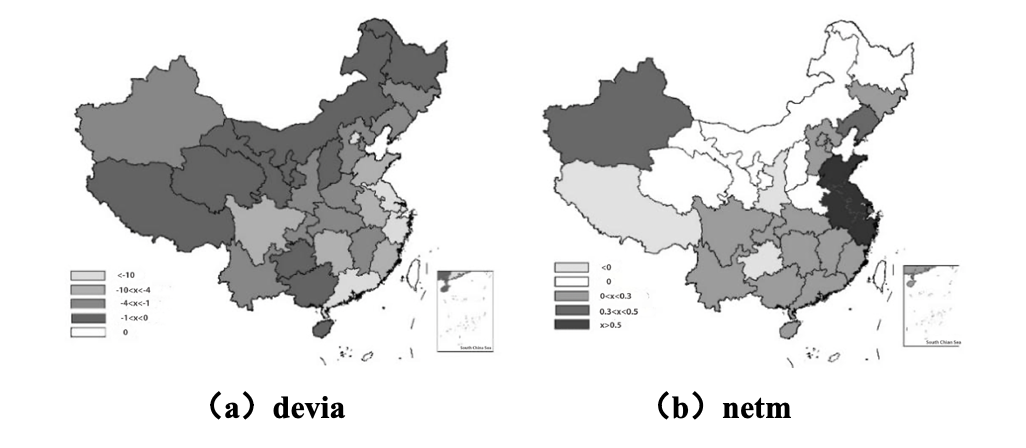
\includegraphics[width=\linewidth]{images/map_ownership.png}
            \captionof{figure}{\tiny Fig 9: Differences in (a) Ownership Separation \& (b) Network Centrality}
        \end{column}
        \begin{column}{0.4\textwidth}
            \begin{alertblock}{Main Finding}
                These maps show the differences in ownership separation (\textit{devia}) and board network centrality (\textit{netm}).
                \begin{itemize}
                    \item DIT firms, particularly in the \textcolor{red}{eastern regions}, tend to exhibit lower ownership separation and higher network centrality.
                \end{itemize}
            \end{alertblock}
        \end{column}
    \end{columns}
\end{frame}

\begin{frame}[fragile]
    \frametitle{Results: Main Effect Regression Table}
    \begin{block}{Table 5: Analysis of Regression Results on TFP}
    \centering
    \setlength{\tabcolsep}{3pt} 
    \tiny
    \begin{tabular}{l c c c c c c c c}
    \toprule
    & \multicolumn{4}{c}{Full Sample DID} & \multicolumn{4}{c}{PSM-DID} \\
    \cmidrule(lr){2-5} \cmidrule(lr){6-9}
    VARIABLES & (1) & (2) & (3) & (4) & (5) & (6) & (7) & (8) \\
    & TFP & TFP & TFP & TFP & TFP & TFP & TFP & TFP \\
    \midrule
    Dit & 0.120*** & 0.093*** & 0.092*** & 0.187*** & 0.040*** & 0.029*** & 0.028*** & 0.022*** \\
    & (20.08) & (20.94) & (20.85) & (20.32) & (8.39) & (9.52) & (9.40) & (8.80) \\
    \\
    Age & & 0.021 & 0.022 & 0.018 & & 0.012 & 0.011 & 0.017 \\
    & & (1.53) & (1.61) & (1.30) & & (0.73) & (0.67) & (1.01) \\
    \\
    Capd & & 0.123*** & 0.123*** & 0.122*** & & 0.325*** & 0.325*** & 0.324*** \\
    & & (96.04) & (96.05) & (95.64) & & (76.74) & (76.69) & (76.44) \\
    \\
    Rese & & -0.014*** & -0.014*** & -0.013*** & & -0.134*** & -0.134*** & -0.143*** \\
    & & (-14.78) & (-14.74) & (-14.00) & & (-3.40) & (-3.37) & (-2.95) \\
    \\
    Controls & No & Yes & Yes & Yes & No & Yes & Yes & Yes \\
    Region Controls & No & No & Yes & Yes & No & No & Yes & Yes \\
    Industry Controls & No & No & No & Yes & No & No & No & Yes \\
    \midrule
    Observations & 45,211 & 45,211 & 44,782 & 44,782 & 33,251 & 33,251 & 33,016 & 33,016 \\
    adj. R2 & 0.679 & 0.774 & 0.776 & 0.778 & 0.650 & 0.748 & 0.750 & 0.752 \\
    \bottomrule
    \end{tabular}
    \end{block}
    \tiny Note: T-statistics in parentheses. *** p<0.01, ** p<0.05, * p<0.1. Firm-level controls include Lern, SA, and Loan.
\end{frame}

\begin{frame}
  \frametitle{Results: Main Effect of DIT on TFP (Summary)}
  \begin{block}{Key Finding (from Table 5, Column 8)}
    DIT has a \textbf{significant and positive} effect on enterprise TFP.
  \end{block}
  \begin{itemize}
    \item The coefficient of the core variable $Dit$ is consistently positive and significant at the 1\% level.
    \item This confirms our main hypothesis (H1).
    \item The robust PSM-DID coefficient is \textbf{0.022***}.
  \end{itemize}
  \begin{alertblock}{Interpretation}
    Implementing DIT, on average, increases a firm's TFP by approximately 2.2\% compared to similar firms that did not.
  \end{alertblock}
\end{frame}

\begin{frame}[fragile]
    \frametitle{Mechanism Test: Governance Personnel Structure}
    \begin{block}{Table 6: Test Results for Personnel Structure}
    \centering
    \tiny
    \begin{tabular}{l c c c c}
    \toprule
    & \multicolumn{2}{c}{Mechanism: Proportion of Female Managers} & \multicolumn{2}{c}{Mechanism: Average Age of Managers} \\
    \cmidrule(lr){2-3} \cmidrule(lr){4-5}
    VARIABLES & (1) fman & (2) TFP & (3) mage & (4) TFP \\
    \midrule
    Dit & \textcolor{red}{0.024***} & 0.176*** & \textcolor{red}{-0.011***} & 0.174*** \\
        & (17.98) & (17.14) & (-11.37) & (17.35) \\
    \\
    Mechanism Var. & & 0.209*** & & 0.040 \\
                   & & (4.28)   & & (0.60) \\
    \midrule
    Mediation Effect & \multicolumn{2}{c}{0.005} & \multicolumn{2}{c}{-0.001} \\
    Sobel Test       & \multicolumn{2}{c}{\textcolor{red}{4.16***}} & \multicolumn{2}{c}{-0.60} \\
    \bottomrule
    \end{tabular}
    \end{block}
    \vfill
    \begin{alertblock}{Interpretation}
        DIT significantly increases the proportion of female executives, which in turn boosts TFP (a significant mediation effect). The effect through management age is not significant in this test.
    \end{alertblock}
\end{frame}

\begin{frame}[fragile]
    \frametitle{Mechanism Test: DSE Compensation}
    \begin{block}{Table 7: Test Results for DSE Compensation}
    \centering
    \tiny
    \begin{tabular}{l c c c c c c}
    \toprule
    & \multicolumn{2}{c}{Director Comp.} & \multicolumn{2}{c}{Supervisor Comp.} & \multicolumn{2}{c}{Executive Comp.} \\
    \cmidrule(lr){2-3} \cmidrule(lr){4-5} \cmidrule(lr){6-7}
    VARIABLES & (1) mwage1 & (2) TFP & (3) mwage2 & (4) TFP & (5) mwage3 & (6) TFP \\
    \midrule
    Dit & \textcolor{red}{0.059***}& 0.146*** & \textcolor{red}{0.101***} & 0.148*** & \textcolor{red}{0.058***} & 0.144*** \\
        & (5.94) & (15.34)  & (7.30)   & (15.31)  & (5.61)   & (15.30) \\
    \\
    Mechanism Var. & & 0.258*** & & 0.101*** & & 0.243*** \\
                   & & (41.54)  & & (21.93)  & & (40.70) \\
    \midrule
    Sobel Test & \multicolumn{2}{c}{\textcolor{red}{5.88***}} & \multicolumn{2}{c}{\textcolor{red}{6.93***}} & \multicolumn{2}{c}{\textcolor{red}{5.56***}} \\
    \bottomrule
    \end{tabular}
    \end{block}
    \vfill
    \begin{alertblock}{Interpretation}
        DIT leads to a significant increase in compensation for directors, supervisors, and executives. All three compensation channels are found to be \textbf{significant mediators} in the DIT-TFP relationship.
    \end{alertblock}
\end{frame}

\begin{frame}[fragile]
    \frametitle{Mechanism Test: Ownership-Control Structure}
    \begin{block}{Table 8: Test Results for Ownership Structure}
    \centering
    \tiny
    \begin{tabular}{l c c c c}
    \toprule
    & \multicolumn{2}{c}{Mechanism: Separation of Ownership} & \multicolumn{2}{c}{Mechanism: Network Centrality} \\
    \cmidrule(lr){2-3} \cmidrule(lr){4-5}
    VARIABLES & (1) devia & (2) TFP & (3) netm & (4) TFP \\
    \midrule
    Dit & \textcolor{red}{-0.096***} & 0.156*** & \textcolor{red}{0.048***} & 0.097*** \\
        & (-5.04) & (10.32) & (10.25) & (8.89) \\
    \\
    Mechanism Var. & & -0.013 & & 0.057*** \\
                   & & (-1.59) & & (3.07) \\
    \midrule
    Sobel Test       & \multicolumn{2}{c}{1.52} & \multicolumn{2}{c}{\textcolor{red}{2.94***}} \\
    \bottomrule
    \end{tabular}
    \end{block}
    \vfill
    \begin{alertblock}{Interpretation}
       DIT significantly reduces ownership separation and increases network centrality. However, only \textbf{network centrality} is found to be a significant mediating pathway.
    \end{alertblock}
\end{frame}

\begin{frame}
  \frametitle{Results: Mechanism Analysis (Summary)}
    \begin{block}{Path 1: Governance Personnel Structure}
        DIT significantly \textbf{increases} the proportion of female managers (coeff: 0.024***) and \textbf{reduces} the average age of managers (coeff: -0.011***). Both are significant mediators.
    \end{block}
    \begin{block}{Path 2: DSE Compensation}
        DIT leads to a significant \textbf{increase} in compensation for directors (0.059***), supervisors (0.101***), and executives (0.058***), all of which are significant mediators.
    \end{block}
    \begin{block}{Path 3: Ownership-Control Structure}
        DIT significantly \textbf{reduces} ownership-control separation (coeff: -0.096***) and \textbf{increases} board network centrality (coeff: 0.048***).
    \end{block}
\end{frame}

\begin{frame}
    \frametitle{Addressing Mediator Endogeneity}
    \begin{block}{The Challenge}
    A key concern is that mediators (e.g., DSE Compensation, Governance Structure) might be endogenous, potentially influenced by unobserved shocks that also affect TFP. This could bias our mediation analysis.
    \end{block}
    <2->
    \begin{alertblock}{The Solution: System GMM}
    We employ the System Generalized Method of Moments (System GMM) to re-estimate the mediation paths. This approach:
    \begin{itemize}
        \item Uses lagged values of variables as internal instruments to mitigate endogeneity.
        \item Accounts for unobserved heterogeneity and dynamic dependencies (i.e., the effect of lagged TFP on current TFP).
    \end{itemize}
    \end{alertblock}
\end{frame}

\begin{frame}[fragile]
    \frametitle{System GMM Results: Mediators Remain Significant}
    \begin{block}{Summary of System GMM tests for Mediator Endogeneity}
    \centering
    \begin{tabular}{l l c}
    \toprule
    \textbf{Mediating Path} & \textbf{Mediating Variable} & \textbf{Effect on TFP (Sys-GMM)} \\
    \midrule
    \textbf{Personnel Structure} & Female Exec. Ratio (\textit{fman}) & \textcolor{red}{0.299***} \\
                                 & Mgmt. Age (\textit{mage}) & \textcolor{red}{-0.241*} \\
    \addlinespace
    \textbf{DSE Compensation} & Director Compensation (\textit{mwage1}) & \textcolor{red}{0.025***} \\
    \addlinespace
    \textbf{Ownership Structure} & Ownership Separation (\textit{devia}) & \textcolor{red}{-0.040***} \\
                                 & Network Centrality (\textit{netm}) & \textcolor{red}{0.178***} \\
    \bottomrule
    \end{tabular}
    \end{block}
    \vfill
    \begin{alertblock}{Conclusion}
    The System GMM results confirm that our key mediating pathways remain \textbf{statistically significant} after addressing potential endogeneity. This strongly supports the robustness of our findings.
    \end{alertblock}
\end{frame}

\begin{frame}
  \frametitle{Results: Heterogeneity and Robustness}
  \begin{columns}[T]
    \begin{column}{0.5\textwidth}
      \begin{block}{Heterogeneity}
        The positive effects of DIT are significantly \textbf{stronger} for:
        \begin{itemize}
          \item Non-State-Owned Enterprises (NSOEs)
          \item Firms in the Eastern Region
          \item Capital-intensive firms
        \end{itemize}
      \end{block}
    \end{column}
    \begin{column}{0.5\textwidth}
      \begin{alertblock}{Robustness Checks}
        Our findings are robust across a series of tests:
        \begin{itemize}
          \item Placebo Test
          \item System GMM
          \item Alternative TFP Measure (LP)
          \item Alternative Matching (1:1)
          \item Synthetic DID (SDID)
        \end{itemize}
      \end{alertblock}
    \end{column}
  \end{columns}
\end{frame}

% --- NEW DETAILED SLIDES ADDED HERE ---
\begin{frame}
    \frametitle{Detailed Results: Heterogeneity Analysis}
    \begin{alertblock}{Finding: The Impact of DIT is Not Uniform}
        The positive effects of DIT on TFP, and the strength of the governance mediation channels, are found to be significantly \textbf{stronger} for:
        \begin{itemize}
            \item \textbf{Non-State-Owned Enterprises (NSOEs)} vs. SOEs.
            \item Firms in the \textbf{Eastern Region} vs. Central/Western regions.
            \item \textbf{Capital-intensive} firms vs. Labor-intensive firms.
        \end{itemize}
        \vfill
        \pause
        This suggests that market orientation, regional infrastructure, and a firm's capital base are crucial moderators that amplify the benefits of DIT.
    \end{alertblock}
\end{frame}

\begin{frame}
    \frametitle{Detailed Robustness Check 1: Alternative Specifications}
    \begin{block}{A Battery of Tests Confirm Our Main Findings}
        In addition to System GMM, the positive and significant effect of DIT on TFP holds when we:
        \begin{itemize}
            \item \textbf{Change the Dependent Variable:} Use the Levinsohn-Petrin (LP) method to calculate TFP. The main coefficient remains significant.
            \item \textbf{Change the DIT Measure:} Use the frequency of keywords as a continuous measure of DIT intensity. Results hold.
            \item \textbf{Change the Matching Method:} Employ a 1:1 nearest neighbor matching instead of 1:2. Results are consistent.
        \end{itemize}
    \end{block}
\end{frame}

\begin{frame}[fragile]
    \frametitle{Detailed Robustness Check 2: Placebo Test}
    \begin{columns}[T]
        \begin{column}{0.5\textwidth}
            \begin{block}{Method}
                We randomly assigned the DIT "treatment" to firms 1000 times and re-ran the regression. This test checks if our result could be due to pure chance.
            \end{block}
            \begin{alertblock}{Result}
                The distribution of the 1000 randomly estimated coefficients is centered around zero. Our actual estimated coefficient (\textcolor{red}{0.022}) is an extreme outlier, indicating that our result is \textbf{not driven by random chance}.
            \end{alertblock}
        \end{column}
        \begin{column}{0.5\textwidth}
            \centering
            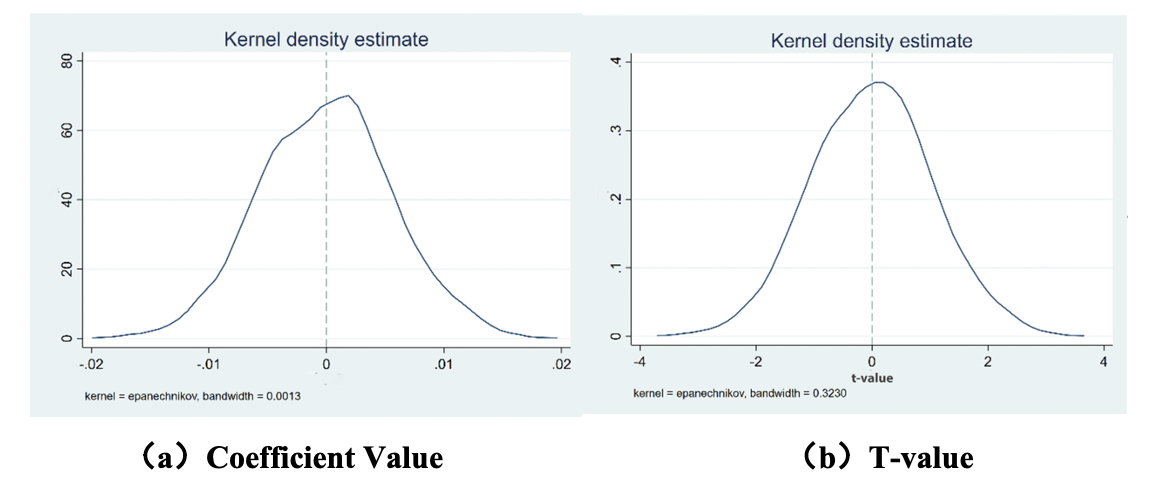
\includegraphics[width=\linewidth]{images/placebo_test.png}
            \captionof{figure}{\tiny Kernel density of estimated coefficients from 1000 placebo runs.}
        \end{column}
    \end{columns}
\end{frame}

\begin{frame}
    \frametitle{Detailed Robustness Check 3: Synthetic DID}
     \begin{columns}[T]
        \begin{column}{0.6\textwidth}
            \centering
            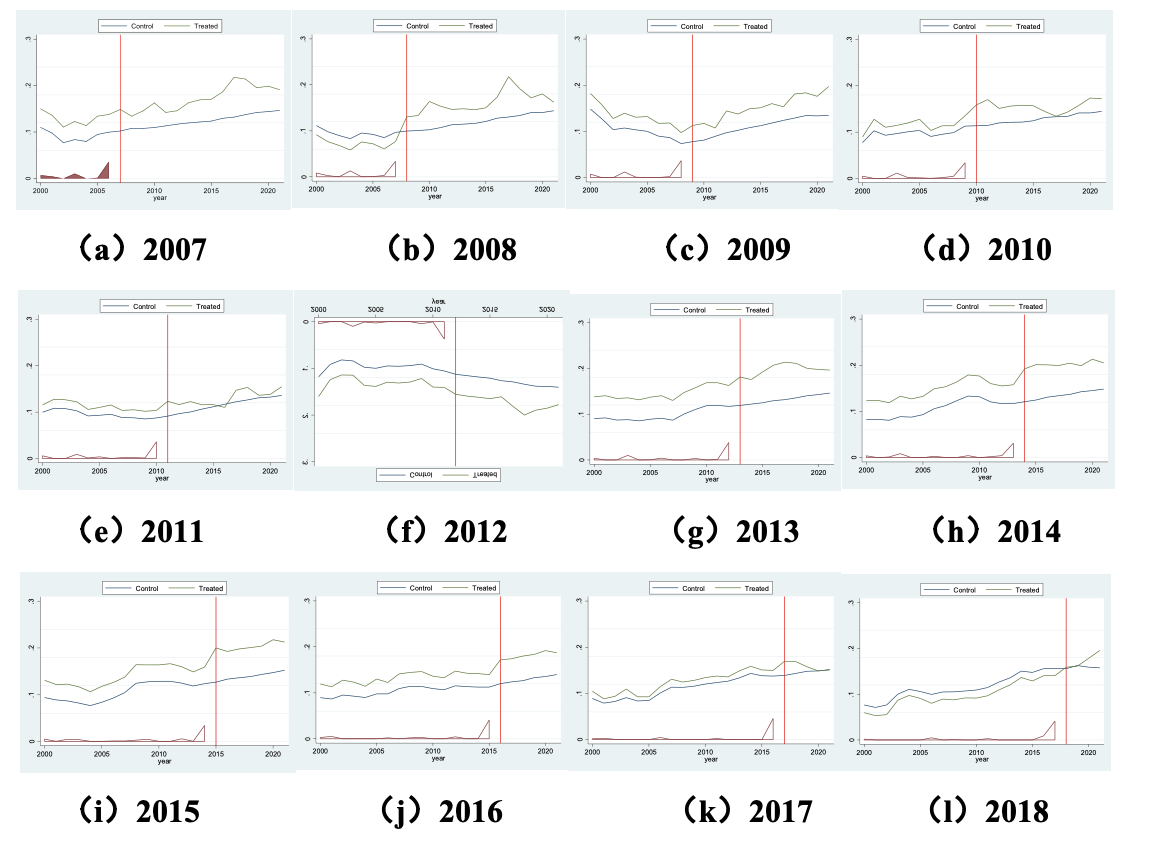
\includegraphics[width=\linewidth]{images/sdid_personnel.png}
            \captionof{figure}{\tiny Example: SDID result for Female Governance Personnel}
        \end{column}
        \begin{column}{0.4\textwidth}
            \begin{block}{Method}
               We use Synthetic DID (Arkhangelsky et al., 2021) to create a better counterfactual for each treated firm, further addressing selection bias.
            \end{block}
            \begin{alertblock}{Result}
               The plots for our key variables, like this one for `fman`, show a clear \textcolor{red}{positive treatment effect} post-DIT, where the treated group's outcome pulls away from its synthetic control.
            \end{alertblock}
        \end{column}
    \end{columns}
\end{frame}
% --- NEW SLIDES END HERE ---

% --- SECTION 5: CONCLUSION ---
\section{Conclusion}

\begin{frame}
  \frametitle{Conclusion and Policy Implications}
    \begin{block}{Key Conclusions}
        \begin{enumerate}
            \item DIT significantly enhances enterprise TFP.
            \item This effect is mediated through the optimization of governance structures: improving personnel, aligning incentives via compensation, and increasing transparency.
            \item The benefits of DIT are context-dependent, being stronger in more market-oriented and technologically advanced firms.
        \end{enumerate}
    \end{block}
    <2->
    \begin{alertblock}{Policy Recommendations}
        \begin{itemize}
            \item Governments should continue to support DIT for SMEs.
            \item Enterprises must innovate management models in parallel with technology adoption.
            \item Refine compensation systems to create clear digital incentives.
        \end{itemize}
    \end{alertblock}
\end{frame}

% --- NEW, HIGH-DENSITY REFERENCES SLIDE ---
% This frame uses multiple techniques to fit ~20 references per slide.
\begin{frame}[allowframebreaks, fragile] % 'fragile' is needed for the font commands
    \frametitle{References}
    
    % This block of commands will ONLY apply to the bibliography
    { 
      \setbeamerfont{bibliography entry author}{size=\tiny}
      \setbeamerfont{bibliography entry title}{size=\tiny}
      \setbeamerfont{bibliography entry location}{size=\tiny}
      \setbeamerfont{bibliography entry note}{size=\tiny}
      \setlength{\bibsep}{0pt} % Removes space between bibliography items
      
      \bibliographystyle{apalike}
      \nocite{*} % Displays all references from the .bib file
      \bibliography{references}
    }
\end{frame}

\begin{frame}
  \frametitle{Thank You!}
  \vfill
  \centering
  \Huge \textbf{Q \& A}
  \vfill
\end{frame}

\end{document}